\chapter{Introduction}

Modern chip multiprocessors (CMPs) rely on Network-on-Chip (NoC) interconnects to support communication between cores, caches, memory controllers, and other peripheral devices. As system sizes scale to tens and even hundreds of cores, NoC become a central component in determining overall system performance, as they directly impact latency, throughput, and scalability \cite{Dally2001}.

With continued technology scaling and prolonged operational stresses induced by demanding CMP worloads, however, reliability has emerged as a major concern. Aging mechanisms such as electromigration (EM) in interconnects and hot-carrier injection (HCI) in transistors degrade components over time. EM primarily affects interconnect wires under high current density and temperature, while HCI degrades transistors based on switching stress \cite{Clotho2015}. In both cases, aging is driven by switching activity, meaning heavily utilized components wear out faster, especially under elevated temperature and process variation. In NoCs, these factors are directly influenced by traffic patterns, making routing decisions a key determinant of how wear accumulates across the network.

\begin{figure}[ht]
  \begin{center}
      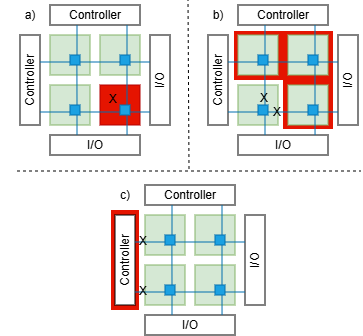
\includegraphics[width=0.95\linewidth]{body_chapters/chap_1/figs/2x2NoCFailure.png}
      \caption[CMP Failure Modes]{4-core CMP with a 2D mesh NoC interconnect. (a) Core failure due to wearout. (b) Router failure due to wearout. (c) Link failure due to wearout.}
      \label{fig:NoC_failure_modes}
  \end{center}
\end{figure}

Wearout in interconnects is particularly concerning because, unlike cores, which can often tolerate failures through redundancy or task remapping, failures in the interconnect are far more critical. As illustrated in Figure \ref{fig:NoC_failure_modes}, while a core failure (Fig. \ref{fig:NoC_failure_modes}a) may degrade performance, router (Fig. \ref{fig:NoC_failure_modes}b) or link failures (Fig. \ref{fig:NoC_failure_modes}c) can disrupt connectivity, partition the network, and render large portions of the system unusable.

Conventional routing algorithms, such as dimension-order routing (DOR), are oblivious to these effects. Their deterministic nature leads to uneven traffic distribution, with central routers and links experiencing consistently higher utilization. This imbalance translates directly into accelerated aging of specific components, effectively reducing the lifetime of the entire network. Prior work on NoC reliability has largely focused on fault-tolerant routing, where the objective is to maintain connectivity in the presence of permanent faults. These approaches are inherently reactive, requiring fault detection and reconfiguration after failures occur \cite{Adnan2025} \cite{Samala2020} \cite{Samala2022}. In contrast, aging-aware routing aims to delay the onset of such failures by controlling how traffic is distributed over time. This class of routing algorithms is fundamentally adaptive: routing decisions are influenced by dynamic metrics such as utilization, temperature, and accumulated wear, with the goal of balancing stress across the network and extending system lifetime.

Existing aging-aware routing techniques typically rely on explicit modeling of path reliability, combining metrics such as EM- and HCI-induced mean time to failure (MTTF) across candidate routes. While effective, these approaches often require global visibility of network state and repeated path evaluation, resulting in significant computational and storage overhead. Furthermore, their reliance on fixed cost functions and heuristics limits their ability to adapt to changing traffic patterns and evolving wear conditions over long execution periods \cite{Clotho2015} \cite{AROMa2018}.

\section{Problem Statement}

Current NoC routing algorithms do not account for long-term aging effects, leading to uneven wear and premature failure of critical components. Existing aging-aware approaches attempt to address this issue but often depend on "piggybacking" global information and fixed heuristics, making them difficult to scale and adapt to dynamic conditions.

This work focuses on developing a routing strategy that can adapt to changing network conditions while remaining lightweight and scalable, with the goal of improving overall system lifetime without significantly impacting performance.

\section{Scope of Research}

This thesis proposes a wear-aware routing approach based on linear approximate reinforcement learning. Instead of explicitly computing path reliability metrics, the routing policy is learned through interaction with the network, allowing the system to implicitly capture the relationship between traffic patterns and aging effects.

The key contributions of this work are:
\begin{itemize}
    \item A reinforcement learning-based aging-aware routing algorithm
    \item Integration of a linear function approximation model that enables scalability and low-overhead implementation at each router
    \item Integration of a deadlock-free adaptive routing design using escape virtual channels
    \item Implementation in the gem5 Garnet NoC simulator and evaluation demonstrating improved lifetime metrics
\end{itemize}